\documentclass[a4paper,12pt]{report}
\usepackage[fiche,niveau={1MA1},nfiche={20}, annee={Emilie-Gourd, 2024--2025},
auteur={ns},theme={Fonctions -- Domaine de définition}]{packages/bandeaux}
\usepackage{packages/boites}
\usepackage{packages/fontes}
\usepackage{packages/courslatex}
\usepackage{packages/mathenv}
\usepackage{tkz-tab}       % For function tables
\allowdisplaybreaks
\renewcommand{\path}{./}
\input{./preambules/print_exo.tex}

\begin{document}
{\bfseries Compétences :}
\begin{itemize}
	\item Réciter la définition du domaine de définition.
	\item Déterminer le domaine de définition d'une fonction racine carrée ou inverse.
\end{itemize}
    
\begin{defi}[Domaine de définition]
	Soit une fonction réelle $f$. Le {\bfseries domaine de définition} de $f$, noté $D_f$, est le sous-ensemble de $\mathbb{R}$ des nombres qui admettent une image par $f$.  
        \[D_f=\{x\in \mathbb{R} \;|\; f(x)\in \mathbb{R}\}.\]
	Ainsi, 
	\[f:D_f\rightarrow \R\]
\end{defi}

\begin{boiteExT}[Déterminons quelques domaines de définition]
\begin{tasks}(2)
	\task[] $f:x\mapsto 3x+2$
	\task[] $g:x\mapsto x^2-1$
	\vspace{2cm}
	\task[] $h:x\mapsto \sqrt{x}$
	\task[] $i:x\mapsto \sqrt[3]{x-1}$
	\vspace{3cm}
	\task[] $j:x\mapsto \dfrac{1}{x-2}$
	\task[] $k:x\mapsto \sqrt{x^2}$
	\vspace{4cm}
	\task[] $\ell:x\mapsto \sqrt{x}^2$
	\vspace{3cm}
\end{tasks}
\vspace{20cm}
\end{boiteExT}
\begin{boiteicone}
	Les fonctions connues pour lesquelles il faut faire attention au domaine de définition sont les fonctions qui contiennent une expression avec la variable au dénominateur ou une racine paire ($\sqrt[2]{},\sqrt[4]{},\ldots$).
\end{boiteicone}
\newpage
{\bfseries Cas 1~: Expression avec une variable au dénominateur}
\medskip

Dans ce cas, on se rappelle que la division par $0$ n'est pas définie. On exclut donc du domaine de définition toutes les valeurs de la variable qui annulent le dénominateur. On ne se soucie pas dans ce cas du numérateur.

\begin{center}
	Déterminer le domaine de définition de $f(x)=\dfrac{3x+1}{4x-3}$
\end{center}
\begin{enumerate}
	\item L'expression contient une variable au dénominateur.
	\item On ne veut jamais être dans le cas d'une division par $0$.
	\item On exclut du domaine de définition les valeurs qui annulent le dénominateur, c'est-à-dire on résout l'équation $4x-3=0$.
	\item On obtient que $4x-3=0\iff x=\dfrac{3}{4}$.
	\item Le domaine de définition est $D_f=\mathbb{R}\setminus\left\{\dfrac{3}{4}\right\}$
\end{enumerate}
	
\insertexo{1M-645w8}{false}{exo}{true}

\medskip

{\bfseries Cas 2~: Expression avec une racine paire (dans notre cas, carrée)}
\medskip 

Dans ce cas, on se rappelle que la racine paire d'un nombre négatif n'est pas définie. On exclut donc du domaine de définition toutes les valeurs de la variable qui entraîne le calcul d'une racine négative. On ne se soucie que de l'expression sous la racine. 
\begin{center}
	Déterminer le domaine de définition de la $f(x)=1+x-\sqrt{2-x^2}$
\end{center}
\begin{enumerate}
	\item La partie de l'expression à considérer est $\sqrt{2-x^2}$
	\item L'expression n'est pas définie lorsque $2-x^2<0$.
	\item $y=2-x^2$ est une parabole concave, donc l'expression est seulement positive pour les valeurs entre les zéros (si la fonction en admet). 
	\item Les zéros sont $-\sqrt{2}$ et $\sqrt{2}$.
		{\small
	\begin{center}
		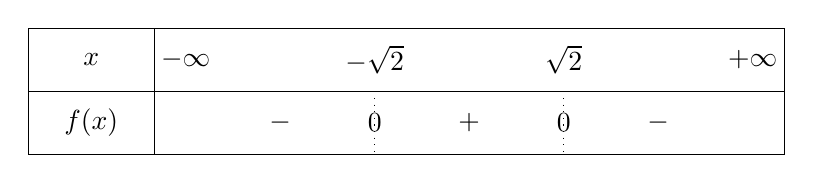
\begin{tikzpicture}[scale=0.8]
			\tkzTabInit{$x$ / 1 , $f(x)$ / 1}{$-\infty$, $-\sqrt{2}$, $\sqrt{2}$, $+\infty$}
			\tkzTabLine{, -, z, +, z, -, }
		\end{tikzpicture}
\end{center}}
\item On exclut du domaine de définition les ensembles $]-\infty;-\sqrt{2}[$ et $]\sqrt{2};+\infty[$. On obtient
	\[D_f=\mathbb{R}\setminus \left(]-\infty;-\sqrt{2}[ \cup ]\sqrt{2};+\infty[\right)=[-\sqrt{2};\sqrt{2}]\]
\end{enumerate}

\medskip

\insertexo{1M-r4ggz}{false}{exo}{true}

\newpage

{\bfseries Cas 3 : Fonction contenant des racines paires et une expression avec une variable au dénominateur}
\smallskip

Dans ce cas, on exclut du domaine de définition toutes les valeurs problématique en menant une étude attentive de la situation.

\begin{boiteExT}[Un exemple plus avancé]
	\begin{center}
		Déterminer le domaine de définition de $f(x)=\dfrac{\sqrt{x-2}}{\sqrt{x+3}}$
	\end{center}
\vspace{15cm}
\end{boiteExT}

\insertexo{1M-v7d64}{false}{exo}{true}

\insertexo{1M-695hr}{false}{exo}{true}

\newpage

\textLigne{Éléments de réponses}
\smallskip

{\footnotesize
	\insertexo{1M-645w8}{false}{cor}{false}

\smallskip
\insertexo{1M-r4ggz}{false}{cor}{false}

\insertexo{1M-v7d64}{false}{cor}{false}
}

\end{document}


